\documentclass[10pt]{beamer}

\usetheme{Berkeley}

% Adding a counter in the bottom of the slide
\setbeamertemplate{page number in head/foot}[framenumber]
\setbeamertemplate{navigation symbols}{\footnotesize\usebeamertemplate{page number in head/foot}}

\usepackage{graphicx}

\begin{document}

\title{Flash Eurozone PMI Analysis}
\author{Hubert Mrugala, Kevin Steijn, Patrick Storz}
\date{December 15, 2020}

% ---------------------------------------------------------------------------
\begin{frame}
\titlepage
\end{frame}
% --------------------------------------------------------------------------
\section{Introduction}
% --------------------------------------------------------------------------
\begin{frame}
\subsection{Team}
\frametitle{Team}

\textbf{Hubert Mrugala} \\
Pursuing a Msc in Banking and Finance at UZH

\vspace{3mm}

\textbf{Kevin Steijn} \\
Pursuing a Msc in Computer Science at UZH

\vspace{3mm}

\textbf{Patrick Storz} \\
Pursuing a Msc in Banking and Finance at UZH 

\end{frame}
% --------------------------------------------------------------------------
\begin{frame}
\subsection{Data}
\frametitle{Data}

We used Worldbank data

\end{frame}
% ----------------------------------------------------------------------------
\section{Analysis}
% --------------------------------------------------------------------------
\begin{frame}
\subsection{European Stock Trends}
\frametitle{European Stock Trends}

\begin{center}
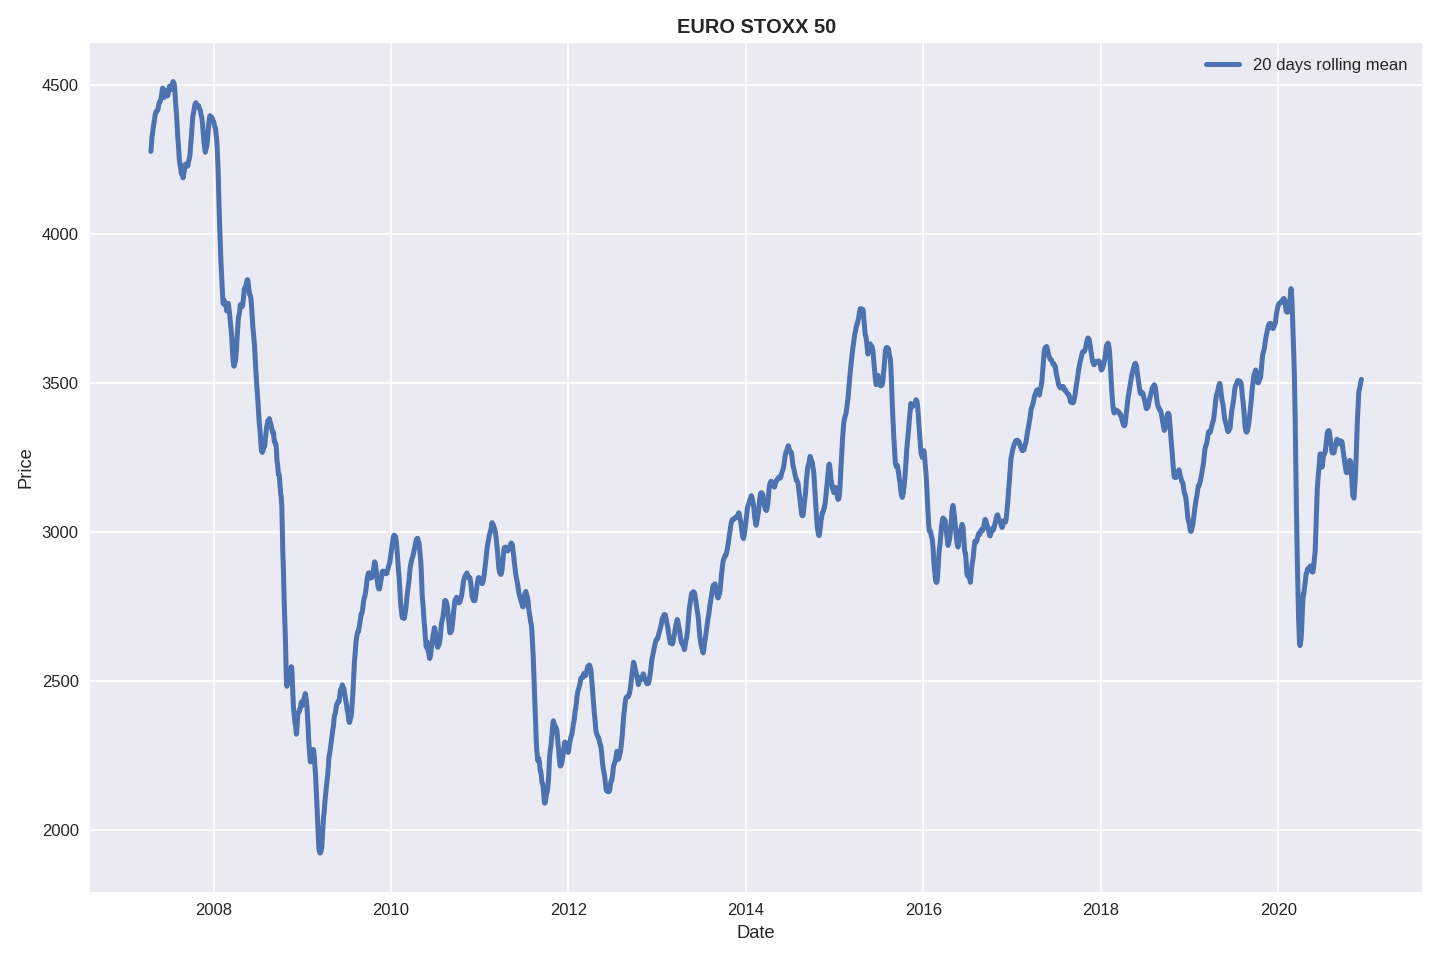
\includegraphics[height=6cm]{STOXX50E.png}
\end{center}

Will the increased volatility continue into 2021?


\end{frame}
% ----------------------------------------------------------------------------
\begin{frame}
\subsection{European Union Growth Trends}
\frametitle{European Union Growth Trends}

\begin{center}
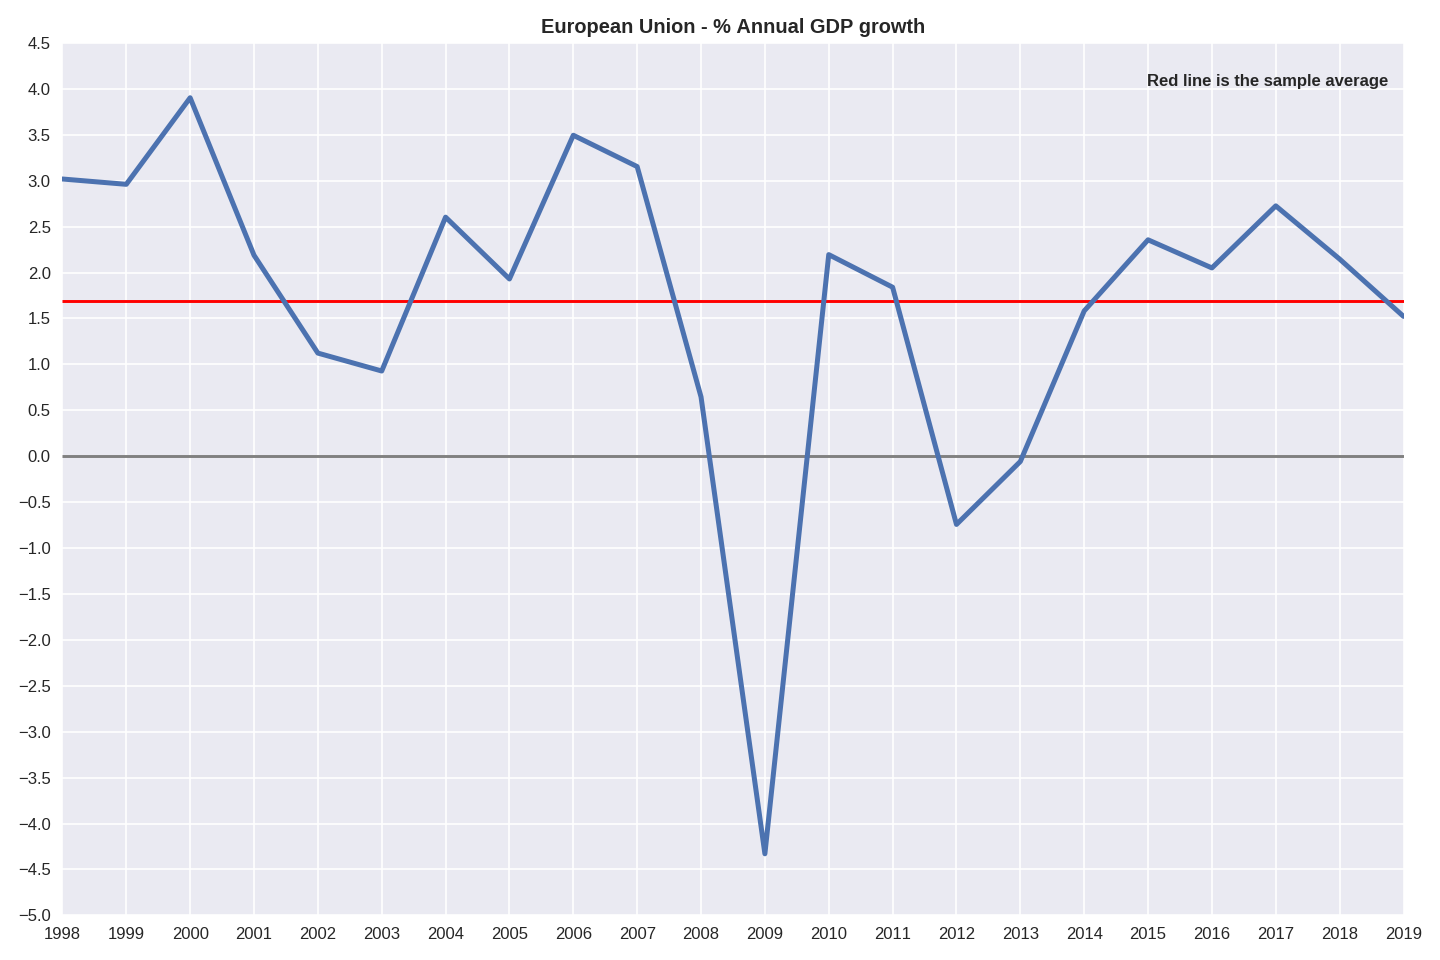
\includegraphics[height=6cm]{EU_GDP.png}
\end{center}

Does the data indicate another decline in growth?

\end{frame}
% ----------------------------------------------------------------------------
\begin{frame}
\subsection{European PMI Values}
\frametitle{European PMI Values}

\begin{center}
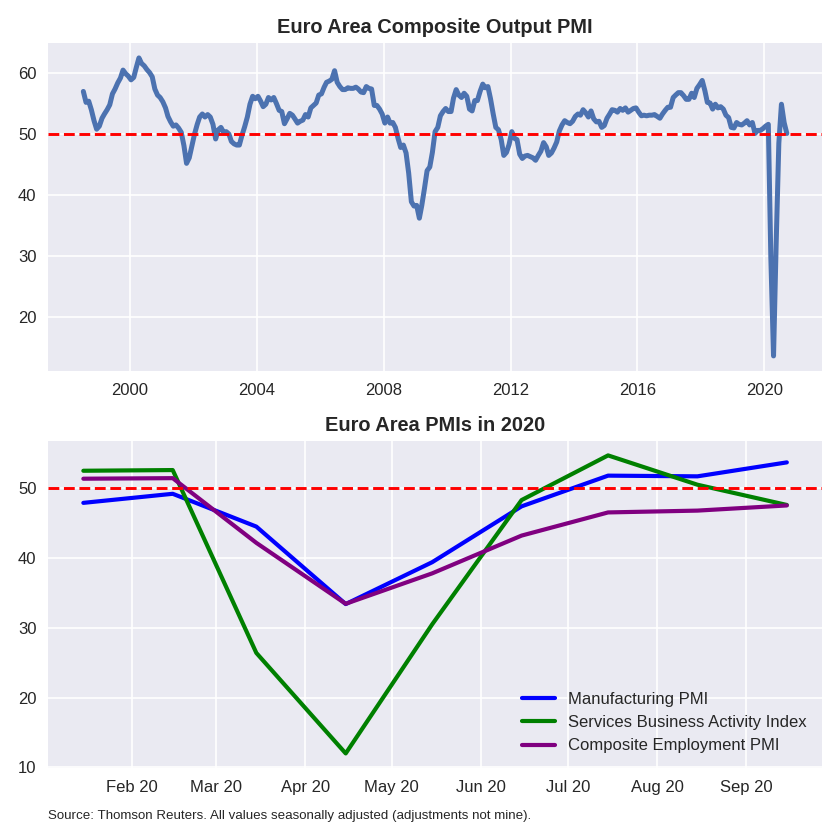
\includegraphics[height=6cm]{PMIs.png}
\end{center}

After a big dive is PMI back to normal?

\end{frame}
% ----------------------------------------------------------------------------
\section{Results}
% --------------------------------------------------------------------------
\begin{frame}
\subsection{Future Research}
\frametitle{Future Research}

PMI will play a role in future research

\end{frame}
% ----------------------------------------------------------------------------
\begin{frame}
\subsection{Conclusion}
\frametitle{Conclusion}

Thanks for your attention

\vspace{1cm}

Any Questions?

\end{frame}
% ----------------------------------------------------------------------------

\end{document}
